\begingroup
\raggedbottom
\setlength{\parskip}{4pt}
\hypersetup{colorlinks=true,linkcolor=appendixink,citecolor=appendixink,urlcolor=appendixink}
\section*{Appendix}
\begin{constructionbox}[title=Reading guide]
\small
\begin{tabularx}{\linewidth}{@{}lXr@{}}
\hyperref[app:families]{A\quad Task catalogue} & Fourteen families, examples and parameters controlling problem size & \pageref{app:families}\\
\hyperref[app:cases]{B\quad Representative constructions} & Four examples from object to score & \pageref{app:cases}\\
\hyperref[app:more]{C\quad Detailed results} & Model comparisons, size--quality curves and sensitivity & \pageref{app:more}\\
\hyperref[app:formats]{D\quad Verification} & Compact formats and algebraic certificates & \pageref{app:formats}\\
\hyperref[app:lit]{E\quad References and bounds} & Literature sources, construction baselines and the LABS target & \pageref{app:lit}\\
\hyperref[app:tiers]{F\quad Instance parameters} & Main and smaller-instance parameter settings & \pageref{app:tiers}\\
\hyperref[app:runner]{G\quad Evaluation settings} & Model settings and an example prompt & \pageref{app:runner}\\
\hyperref[app:tools]{H\quad Code and web access} & Tool-assisted results and token usage & \pageref{app:tools}
\end{tabularx}
\end{constructionbox}
\section{Task catalogue}
\label{app:families}
Each family page gives the objective, a checked small example, parameters controlling problem size and one evaluated instance with its reference values. Small diagrams illustrate the mathematical property. In the tables, the baseline is the better of an implemented mathematical construction and the ten-second search result. It can be weaker than a published frontier, which remains the scoring reference. The final column gives this baseline's relative quality, rather than a model score. Gap closed uses the scoring reference as its starting point, as defined in Section~\ref{sec:headroom}.
\begin{center}\small\setlength{\tabcolsep}{3pt}
\begin{tabularx}{\linewidth}{@{}P{.16\linewidth}YP{.12\linewidth}P{.09\linewidth}P{.22\linewidth}@{}}
\toprule
family & construction & objective & class & reference; bound or target \\
\midrule
\hyperref[family:capset]{cap set} & $S \subseteq \mathbb{F}_3^d$; no three collinear points (cap set) & $|S|$ & R & published; proven bound \\
\hyperref[family:spherical_code]{spherical codes} & vectors with exact coordinates; pairwise angle $\ge\theta$; $60^\circ$ or variable & count & R & mixed; proven bound \\
\hyperref[family:matmul]{matrix multiplication} & bilinear scheme for $(n\times m)$ by $(m\times p)$ matrices; computes the product exactly & rank $r$ (min) & S & published; proven bound \\
\hyperref[family:degdiam]{degree--diameter} & graph with max degree $d$; diameter $\le k$ & vertices & S & published; proven bound \\
\hyperref[family:covering]{covering} & $k$-subsets (blocks) of $[v]$; every $t$-subset lies in a block & blocks (min) & S & published; proven bound \\
\hyperref[family:schur]{Schur} & $k$-colouring of $\{1..N\}$; no monochromatic $x, y, x{+}y$ & $N$ & R & published; proven bound \\
\hyperref[family:apfree_q]{$\mathbb{F}_q^n$ AP-free} & $S \subseteq \mathbb{F}_q^n$, $q\in\{5,7\}$; no 3-term progression & $|S|$ & R & mixed; proven bound \\
\hyperref[family:mols]{MOLS} & Latin squares of order $n$, $n$ not a prime power; pairwise orthogonal & number of squares & R & published; proven bound \\
\midrule
\hyperref[family:labs]{LABS} & $\pm1$ sequence of length $N$; well-formed sequence & merit factor & S & construction; conjectured target \\
\hyperref[family:heilbronn]{Heilbronn} & $n$ points in a square or triangle; distinct points in the domain & min triangle area & S & construction; trivial bound \\
\hyperref[family:corners]{corners} & $S \subseteq [n]^2$; no corner & $|S|$ & R & construction; trivial bound \\
\hyperref[family:lineq]{linear-equation-free} & $S \subseteq \{1..n\}$; no non-trivial solution of the specified linear equation & $|S|$ & R & construction; trivial bound \\
\hyperref[family:shannon]{Shannon} & code in $\{0,\ldots,q-1\}^d$; every pair separates on the cycle & $|C|$ & R & construction; proven bound \\
\hyperref[family:trifference]{trifference} & ternary code of length $n$; every triple has at least $m$ coordinates with three distinct symbols & $|C|$ & U & construction; proven bound \\
\bottomrule
\end{tabularx}

\captionof{table}{The fourteen families. R denotes search-resistant, S families that can benefit from search and U unclassified search sensitivity. These labels concern the reference search procedures studied here. Spherical codes and Heilbronn each contain two variants. Reference types may depend on the parameters.}
\label{tab:families}
\end{center}
\appendixpage
\begin{minipage}{\linewidth}
\catalogueheading{capset}{Cap sets}
A large set must avoid every three-point arithmetic progression. \citep{edel2004capset,karapetyan2023caps}\par\smallskip
\begin{minipage}[c]{.25\linewidth}\centering

\includegraphics[width=.92\linewidth,height=73pt,keepaspectratio]{figs/appendix/capset.pdf}
\par{\scriptsize $d=2$: four points}\end{minipage}\hfill
\begin{minipage}[c]{.71\linewidth}
Maximise $|S|$ for $S\subseteq\mathbb F_3^d$ containing no three distinct points $x,y,z$ with $x+y+z=0$.\par\smallskip
\end{minipage}\par\smallskip
\textbf{Parameters and scaling.} Increasing $d$ enlarges the ambient space to $3^d$ points. Products lift finite caps to higher dimensions.
\begin{resultbox}[top=4pt,bottom=4pt]\small
\textbf{Evaluated example:} $d=10$.\par
\begin{tabularx}{\linewidth}{@{}XXXXX@{}}
Baseline & 10 s search & Reference & Bound or target & Baseline\textquotesingle s relative quality \\
2240 & 1140 & 2432 & 5619 & 0.921 \\
\end{tabularx}\par{\scriptsize Reference: published frontier; proven bound.}\par\smallskip
\end{resultbox}\end{minipage}
\par\vfill
\begin{minipage}{\linewidth}
\catalogueheading{corners}{Corner-free sets}
A dense grid set must avoid a prescribed three-point pattern. \citep{behrend1946}\par\smallskip
\begin{minipage}[c]{.25\linewidth}\centering

\includegraphics[width=.92\linewidth,height=73pt,keepaspectratio]{figs/appendix/corners.pdf}
\par{\scriptsize $n=5$: nine points}\end{minipage}\hfill
\begin{minipage}[c]{.71\linewidth}
Maximise $|S|$ for $S\subseteq\{0,\ldots,n-1\}^2$ containing no triple $(x,y),(x+t,y),(x,y+t)$ with $t\ne0$, including negative $t$.\par\smallskip
\end{minipage}\par\smallskip
\textbf{Parameters and scaling.} Increasing $n$ enlarges the grid. Progression-free difference sets supply constructions at many sizes.
\begin{resultbox}[top=4pt,bottom=4pt]\small
\textbf{Evaluated example:} $n=138$.\par
\begin{tabularx}{\linewidth}{@{}XXXXX@{}}
Baseline & 10 s search & Reference & Bound or target & Baseline\textquotesingle s relative quality \\
3120 & 2504 & 3120 & 19044 & 1.000 \\
\end{tabularx}\par{\scriptsize Reference: construction baseline; trivial bound.}\par\smallskip
\end{resultbox}\end{minipage}
\par\vfill
\appendixpage
\begin{minipage}{\linewidth}
\catalogueheading{schur}{Schur colourings}
No solution to $x+y=z$ may lie entirely within one colour class. \citep{rowley2021templates,bengone2026schur}\par\smallskip
\begin{minipage}[c]{.25\linewidth}\centering
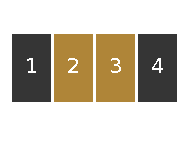
\includegraphics[width=.92\linewidth,height=73pt,keepaspectratio]{figs/appendix/schur.pdf}
\par{\scriptsize $k=2,\ N=4$}\end{minipage}\hfill
\begin{minipage}[c]{.71\linewidth}
Maximise $N$ such that $\{1,\ldots,N\}$ can be coloured with $k$ colours without a monochromatic solution of $x+y=z$. Solutions with $x=y$ are also forbidden.\par\smallskip
\end{minipage}\par\smallskip
\textbf{Parameters and scaling.} Increasing the number of colours $k$ gives new extremal targets. Recursive templates extend smaller colourings.
\begin{resultbox}[top=4pt,bottom=4pt]\small
\textbf{Evaluated example:} $k=7$.\par
\begin{tabularx}{\linewidth}{@{}XXXXX@{}}
Baseline & 10 s search & Reference & Bound or target & Baseline\textquotesingle s relative quality \\
1093 & 1093 & 1696 & 13699 & 0.644 \\
\end{tabularx}\par{\scriptsize Reference: published frontier; proven bound.}\par\smallskip
\end{resultbox}\end{minipage}
\par\vfill
\begin{minipage}{\linewidth}
\catalogueheading{apfree_q}{Progression-free sets over finite fields}
The ambient field changes which additive patterns a set must avoid. \citep{edel_caps,ellenberg2017capset}\par\smallskip
\begin{minipage}[c]{.25\linewidth}\centering

\includegraphics[width=.92\linewidth,height=73pt,keepaspectratio]{figs/appendix/apfree_q.pdf}
\par{\scriptsize $q=5,\ n=2$}\end{minipage}\hfill
\begin{minipage}[c]{.71\linewidth}
Maximise $|S|$ for $S\subseteq\mathbb F_q^n$ containing no three distinct points satisfying $x+z=2y$.\par\smallskip
\end{minipage}\par\smallskip
\textbf{Parameters and scaling.} Varying $q$ or $n$ changes the task. Products and algebraic constructions give candidates across dimensions.
\begin{resultbox}[top=4pt,bottom=4pt]\small
\textbf{Evaluated example:} $q=5,\ n=6$.\par
\begin{tabularx}{\linewidth}{@{}XXXXX@{}}
Baseline & 10 s search & Reference & Bound or target & Baseline\textquotesingle s relative quality \\
360 & 360 & 649 & 7497 & 0.555 \\
\end{tabularx}\par{\scriptsize Reference: published frontier; proven bound.}\par\smallskip
\end{resultbox}\end{minipage}
\par\vfill
\appendixpage
\begin{minipage}{\linewidth}
\catalogueheading{spherical_code}{Spherical codes}
Directions must remain separated while as many vectors as possible are packed. \citep{zinoviev1999contact,ganzhinov2025lines,cohn2003kissing}\par\smallskip
\begin{minipage}[c]{.25\linewidth}\centering
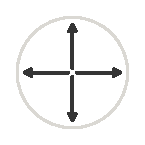
\includegraphics[width=.92\linewidth,height=73pt,keepaspectratio]{figs/appendix/spherical_code.pdf}
\par{\scriptsize $d=2$: four directions}\end{minipage}\hfill
\begin{minipage}[c]{.71\linewidth}
\textbf{Fixed angle.} Maximise the number of nonzero vectors whose pairwise angles are at least $60^\circ$. After normalisation these give a kissing configuration. Coordinates are integers in $[-1000,1000]$; at $d=13$, we also allow $a+b\sqrt3$ with integer $|a|,|b|\le1000$.\par\smallskip
\textbf{Variable angle.} Maximise the number of nonzero vectors in $\mathbb Z^d$ satisfying $u\cdot v\le c\|u\|\|v\|$ for every distinct pair. Coordinates lie in $[-1000,1000]$, and the prescribed rational value $c=\cos\theta$ is checked exactly.\par\smallskip
\end{minipage}\par\smallskip
\textbf{Parameters and scaling.} Dimension $d$ and the angle threshold control the packing problem. Lattices, orbits and signed supports supply constructions.
\begin{resultbox}[top=4pt,bottom=4pt]\small
\textbf{Evaluated example:} $d=14$.\par
\begin{tabularx}{\linewidth}{@{}XXXXX@{}}
Baseline & 10 s search & Reference & Bound or target & Baseline\textquotesingle s relative quality \\
1932 & 876 & 1932 & 3174 & 1.000 \\
\end{tabularx}\par{\scriptsize Reference: published frontier; proven bound.}\par\smallskip
\textbf{Evaluated example:} $d=12,\ c=24/100$.\par
\begin{tabularx}{\linewidth}{@{}XXXXX@{}}
Baseline & 10 s search & Reference & Bound or target & Baseline\textquotesingle s relative quality \\
28 & 24 & 28 & 1431 & 1.000 \\
\end{tabularx}\par{\scriptsize Reference: construction baseline; proven bound.}\par\smallskip
\end{resultbox}\end{minipage}
\par\vfill
\begin{minipage}{\linewidth}
\catalogueheading{labs}{Low-autocorrelation binary sequences}
A binary sequence should have low autocorrelation at nonzero shifts. \citep{packebusch2016labs}\par\smallskip
\begin{minipage}[c]{.25\linewidth}\centering
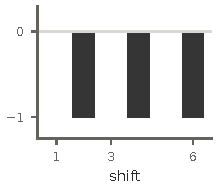
\includegraphics[width=.92\linewidth,height=73pt,keepaspectratio]{figs/appendix/labs.pdf}
\par{\scriptsize $N=7$: autocorrelation}\end{minipage}\hfill
\begin{minipage}[c]{.71\linewidth}
Choose $s\in\{-1,1\}^N$ to maximise the merit factor $N^2/(2\sum_{k=1}^{N-1}C_k^2)$, where $C_k=\sum_{i=1}^{N-k}s_i s_{i+k}$ is the aperiodic autocorrelation.\par\smallskip
\end{minipage}\par\smallskip
\textbf{Parameters and scaling.} Increasing $N$ tests whether a construction retains a high merit factor at longer lengths.
\begin{resultbox}[top=4pt,bottom=4pt]\small
\textbf{Evaluated example:} $N=280$.\par
\begin{tabularx}{\linewidth}{@{}XXXXX@{}}
Baseline & 10 s search & Reference & Bound or target & Baseline\textquotesingle s relative quality \\
5.57769 & 4.4708 & 5.57769 & 12.32 & 1.000 \\
\end{tabularx}\par{\scriptsize Reference: construction baseline; conjectured target.}\par\smallskip
\end{resultbox}\end{minipage}
\par\vfill
\appendixpage
\begin{minipage}{\linewidth}
\catalogueheading{heilbronn}{Heilbronn triangles}
Place the points so that the smallest triangle area is as large as possible. (definitions and references in Appendix~\ref{app:lit})\par\smallskip
\begin{minipage}[c]{.25\linewidth}\centering
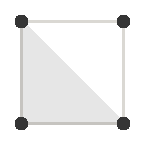
\includegraphics[width=.92\linewidth,height=73pt,keepaspectratio]{figs/appendix/heilbronn.pdf}
\par{\scriptsize $n=4$: minimum area $1/2$}\end{minipage}\hfill
\begin{minipage}[c]{.71\linewidth}
\textbf{Square.} Place $n$ distinct points in $[0,1]^2$ to maximise the smallest area of a triangle determined by three points. Coordinates are multiples of $10^{-4}$.\par\smallskip
\textbf{Triangle.} Place $n$ distinct integer-grid points in a specified triangle $T$ to maximise the smallest triangle area, divided by the area of $T$.\par\smallskip
\end{minipage}\par\smallskip
\textbf{Parameters and scaling.} Increasing $n$ introduces more triangle constraints. The square and triangular domains are evaluated separately.
\begin{resultbox}[top=4pt,bottom=4pt]\small
\textbf{Evaluated example:} $n=46$.\par
\begin{tabularx}{\linewidth}{@{}XXXXX@{}}
Baseline & 10 s search & Reference & Bound or target & Baseline\textquotesingle s relative quality \\
0.00047375 & 0.00047375 & 0.00047375 & 0.0227273 & 1.000 \\
\end{tabularx}\par{\scriptsize Reference: construction baseline; trivial bound.}\par\smallskip
\textbf{Evaluated example:} $n=32$, triangular domain (Table~\ref{tab:triangle_domains}).\par
\begin{tabularx}{\linewidth}{@{}XXXXX@{}}
Baseline & 10 s search & Reference & Bound or target & Baseline\textquotesingle s relative quality \\
0.0014885 & 0.0014885 & 0.0014885 & 0.0333333 & 1.000 \\
\end{tabularx}\par{\scriptsize Reference: construction baseline; trivial bound.}\par\smallskip
\end{resultbox}\end{minipage}
\par\vfill
\begin{minipage}{\linewidth}
\catalogueheading{degdiam}{Degree--diameter graphs}
A sparse graph must keep all vertices close to one another. \citep{miller2013degdiam,comellas_degdiam}\par\smallskip
\begin{minipage}[c]{.25\linewidth}\centering

\includegraphics[width=.92\linewidth,height=73pt,keepaspectratio]{figs/appendix/degdiam.pdf}
\par{\scriptsize $d=2,\ k=2,\ N=5$}\end{minipage}\hfill
\begin{minipage}[c]{.71\linewidth}
Maximise the number of vertices of a simple connected undirected graph with maximum degree at most $d$ and diameter at most $k$.\par\smallskip
\end{minipage}\par\smallskip
\textbf{Parameters and scaling.} Varying degree $d$ and diameter $k$ generates new graph problems. Larger diameters test the growth of a construction.
\begin{resultbox}[top=4pt,bottom=4pt]\small
\textbf{Evaluated example:} $d=4,\ k=5$.\par
\begin{tabularx}{\linewidth}{@{}XXXXX@{}}
Baseline & 10 s search & Reference & Bound or target & Baseline\textquotesingle s relative quality \\
61 & 61 & 364 & 485 & 0.168 \\
\end{tabularx}\par{\scriptsize Reference: published frontier; proven bound.}\par\smallskip
\end{resultbox}\end{minipage}
\par\vfill
\appendixpage
\begin{minipage}{\linewidth}
\catalogueheading{lineq}{Linear-equation-free sets}
A large integer set must avoid a specified linear relation. \citep{behrend1946,ruzsa1993lineq}\par\smallskip
\begin{minipage}[c]{.25\linewidth}\centering
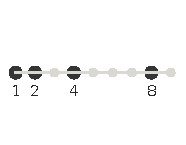
\includegraphics[width=.92\linewidth,height=73pt,keepaspectratio]{figs/appendix/lineq.pdf}
\par{\scriptsize $a=b=1,\ n=9$}\end{minipage}\hfill
\begin{minipage}[c]{.71\linewidth}
Maximise $|S|$ for $S\subseteq\{1,\ldots,n\}$ such that $ax+by=(a+b)z$ has no solution in $S$ except $x=y=z$.\par\smallskip
\end{minipage}\par\smallskip
\textbf{Parameters and scaling.} The coefficients $a,b$ select the relation; $n$ sets the interval size. Digit constructions can extend to larger intervals.
\begin{resultbox}[top=4pt,bottom=4pt]\small
\textbf{Evaluated example:} $a=3,\ b=4,\ n=19044$.\par
\begin{tabularx}{\linewidth}{@{}XXXXX@{}}
Baseline & 10 s search & Reference & Bound or target & Baseline\textquotesingle s relative quality \\
630 & 630 & 630 & 19044 & 1.000 \\
\end{tabularx}\par{\scriptsize Reference: construction baseline; trivial bound.}\par\smallskip
\end{resultbox}\end{minipage}
\par\vfill
\begin{minipage}{\linewidth}
\catalogueheading{covering}{Covering designs}
A small collection of blocks must cover every required subset. \citep{gordon1995covering,ljcr}\par\smallskip
\begin{minipage}[c]{.25\linewidth}\centering
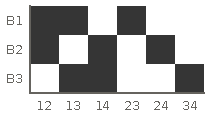
\includegraphics[width=.92\linewidth,height=73pt,keepaspectratio]{figs/appendix/covering.pdf}
\par{\scriptsize Three blocks cover six pairs}\end{minipage}\hfill
\begin{minipage}[c]{.71\linewidth}
Minimise the number of $k$-element blocks drawn from a $v$-element set such that every $t$-element subset is contained in at least one block.\par\smallskip
\end{minipage}\par\smallskip
\textbf{Parameters and scaling.} The parameters $(v,k,t)$ control the universe, block size and subsets to cover. Larger settings test covering efficiency.
\begin{resultbox}[top=4pt,bottom=4pt]\small
\textbf{Evaluated example:} $v=18,\ k=7,\ t=4$.\par
\begin{tabularx}{\linewidth}{@{}XXXXX@{}}
Baseline & 10 s search & Reference & Bound or target & Baseline\textquotesingle s relative quality \\
179 & 179 & 126 & 111 & 0.704 \\
\end{tabularx}\par{\scriptsize Reference: published frontier; proven bound.}\par\smallskip
\end{resultbox}\end{minipage}
\par\vfill
\appendixpage
\begin{minipage}{\linewidth}
\catalogueheading{matmul}{Matrix multiplication}
A bilinear construction reduces the number of scalar multiplications. \citep{strassen1969,fawzi2022alphatensor}\par\smallskip
\begin{minipage}[c]{.25\linewidth}\centering
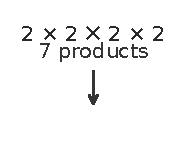
\includegraphics[width=.92\linewidth,height=73pt,keepaspectratio]{figs/appendix/matmul.pdf}
\par{\scriptsize Strassen: seven products}\end{minipage}\hfill
\begin{minipage}[c]{.71\linewidth}
Minimise the number $r$ of scalar multiplications in a bilinear algorithm for $A\in\mathbb R^{n\times m}$ and $B\in\mathbb R^{m\times p}$. The identity $AB=\sum_{j=1}^r (u_j\cdot A)(v_j\cdot B)W_j$ must hold for all inputs, with each dot product taken over matrix entries. Coefficients are integers in $[-4,4]$.\par\smallskip
\end{minipage}\par\smallskip
\textbf{Parameters and scaling.} Changing the matrix dimensions $(n,m,p)$ defines new multiplication problems. Block composition extends schemes to larger products.
\begin{resultbox}[top=4pt,bottom=4pt]\small
\textbf{Evaluated example:} $n=4,\ m=4,\ p=5$.\par
\begin{tabularx}{\linewidth}{@{}XXXXX@{}}
Baseline & 10 s search & Reference & Bound or target & Baseline\textquotesingle s relative quality \\
72 & 72 & 61 & 20 & 0.847 \\
\end{tabularx}\par{\scriptsize Reference: published frontier; proven bound.}\par\smallskip
\end{resultbox}\end{minipage}
\par\vfill
\begin{minipage}{\linewidth}
\catalogueheading{mols}{Mutually orthogonal Latin squares}
When any two squares are superimposed, every ordered pair of symbols must occur exactly once. \citep{miller2024mols,abel2015mols}\par\smallskip
\begin{minipage}[c]{.25\linewidth}\centering
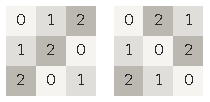
\includegraphics[width=.92\linewidth,height=73pt,keepaspectratio]{figs/appendix/mols.pdf}
\par{\scriptsize Two squares of order three}\end{minipage}\hfill
\begin{minipage}[c]{.71\linewidth}
Find as many mutually orthogonal Latin squares of order $n$ as possible. Each symbol appears once in every row and column; superimposing any two squares must give all $n^2$ ordered symbol pairs exactly once.\par\smallskip
\end{minipage}\par\smallskip
\textbf{Parameters and scaling.} Changing the order $n$ changes the design problem. Algebraic constructions and combinations of smaller designs supply candidates.
\begin{resultbox}[top=4pt,bottom=4pt]\small
\textbf{Evaluated example:} $n=14$.\par
\begin{tabularx}{\linewidth}{@{}XXXXX@{}}
Baseline & 10 s search & Reference & Bound or target & Baseline\textquotesingle s relative quality \\
4 & 1 & 4 & 12 & 1.000 \\
\end{tabularx}\par{\scriptsize Reference: published frontier; proven bound.}\par\smallskip
\end{resultbox}\end{minipage}
\par\vfill
\appendixpage
\begin{minipage}{\linewidth}
\catalogueheading{shannon}{Shannon codes}
In the cycle model, adjacent symbols can be confused; every pair of codewords must have a coordinate that distinguishes them. \citep{lovasz1979shannon,polak2019shannon}\par\smallskip
\begin{minipage}[c]{.25\linewidth}\centering

\includegraphics[width=.92\linewidth,height=73pt,keepaspectratio]{figs/appendix/shannon.pdf}
\par{\scriptsize $C_5^2$: five codewords}\end{minipage}\hfill
\begin{minipage}[c]{.71\linewidth}
Maximise the size of a code $C\subseteq\mathbb Z_q^d$ such that every two distinct words differ by cyclic distance at least two in some coordinate. Equivalently, $C$ is an independent set in the $d$-fold strong power of the cycle $C_q$.\par\smallskip
\end{minipage}\par\smallskip
\textbf{Parameters and scaling.} The cycle size $q$ and codeword length $d$ define the task. Finite factors give short certificates for very large products.
\begin{resultbox}[top=4pt,bottom=4pt]\small
\textbf{Evaluated example:} $q=7,\ d=24$.\par
\begin{tabularx}{\linewidth}{@{}XXXXX@{}}
Baseline & 10 s search & Reference & Bound or target & Baseline\textquotesingle s relative quality \\
$1.9411\times10^{12}$ & $1.9411\times10^{12}$ & $1.9411\times10^{12}$ & $3.16219\times10^{12}$ & 1.000 \\
\end{tabularx}\par{\scriptsize Reference: construction baseline; proven bound.}\par\smallskip
\end{resultbox}\end{minipage}
\par\vfill
\begin{minipage}{\linewidth}
\catalogueheading{trifference}{Trifference codes}
Every triple of distinct codewords must display all three symbols in at least $m$ coordinates. \citep{bishnoi2024trifferent,bishnoi2025generalized}\par\smallskip
\begin{minipage}[c]{.25\linewidth}\centering
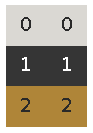
\includegraphics[width=.92\linewidth,height=73pt,keepaspectratio]{figs/appendix/trifference.pdf}
\par{\scriptsize $n=2,\ m=2$: three words}\end{minipage}\hfill
\begin{minipage}[c]{.71\linewidth}
Maximise the size of a ternary code $C\subseteq\{0,1,2\}^n$ such that, for every three distinct words, at least $m$ coordinates contain all three symbols.\par\smallskip
\end{minipage}\par\smallskip
\textbf{Parameters and scaling.} Length $n$ and separation multiplicity $m$ define the task. Linear and concatenated codes admit compact certificates.
\begin{resultbox}[top=4pt,bottom=4pt]\small
\textbf{Evaluated example:} $n=64,\ m=1$.\par
\begin{tabularx}{\linewidth}{@{}XXXXX@{}}
Baseline & 10 s search & Reference & Bound or target & Baseline\textquotesingle s relative quality \\
19683 & 19683 & 19683 & $3.72281\times10^{11}$ & 1.000 \\
\end{tabularx}\par{\scriptsize Reference: construction baseline; proven bound.}\par\smallskip
\end{resultbox}\end{minipage}
\par\vfill

